\begin{figure*}[!ht]
    \centering
    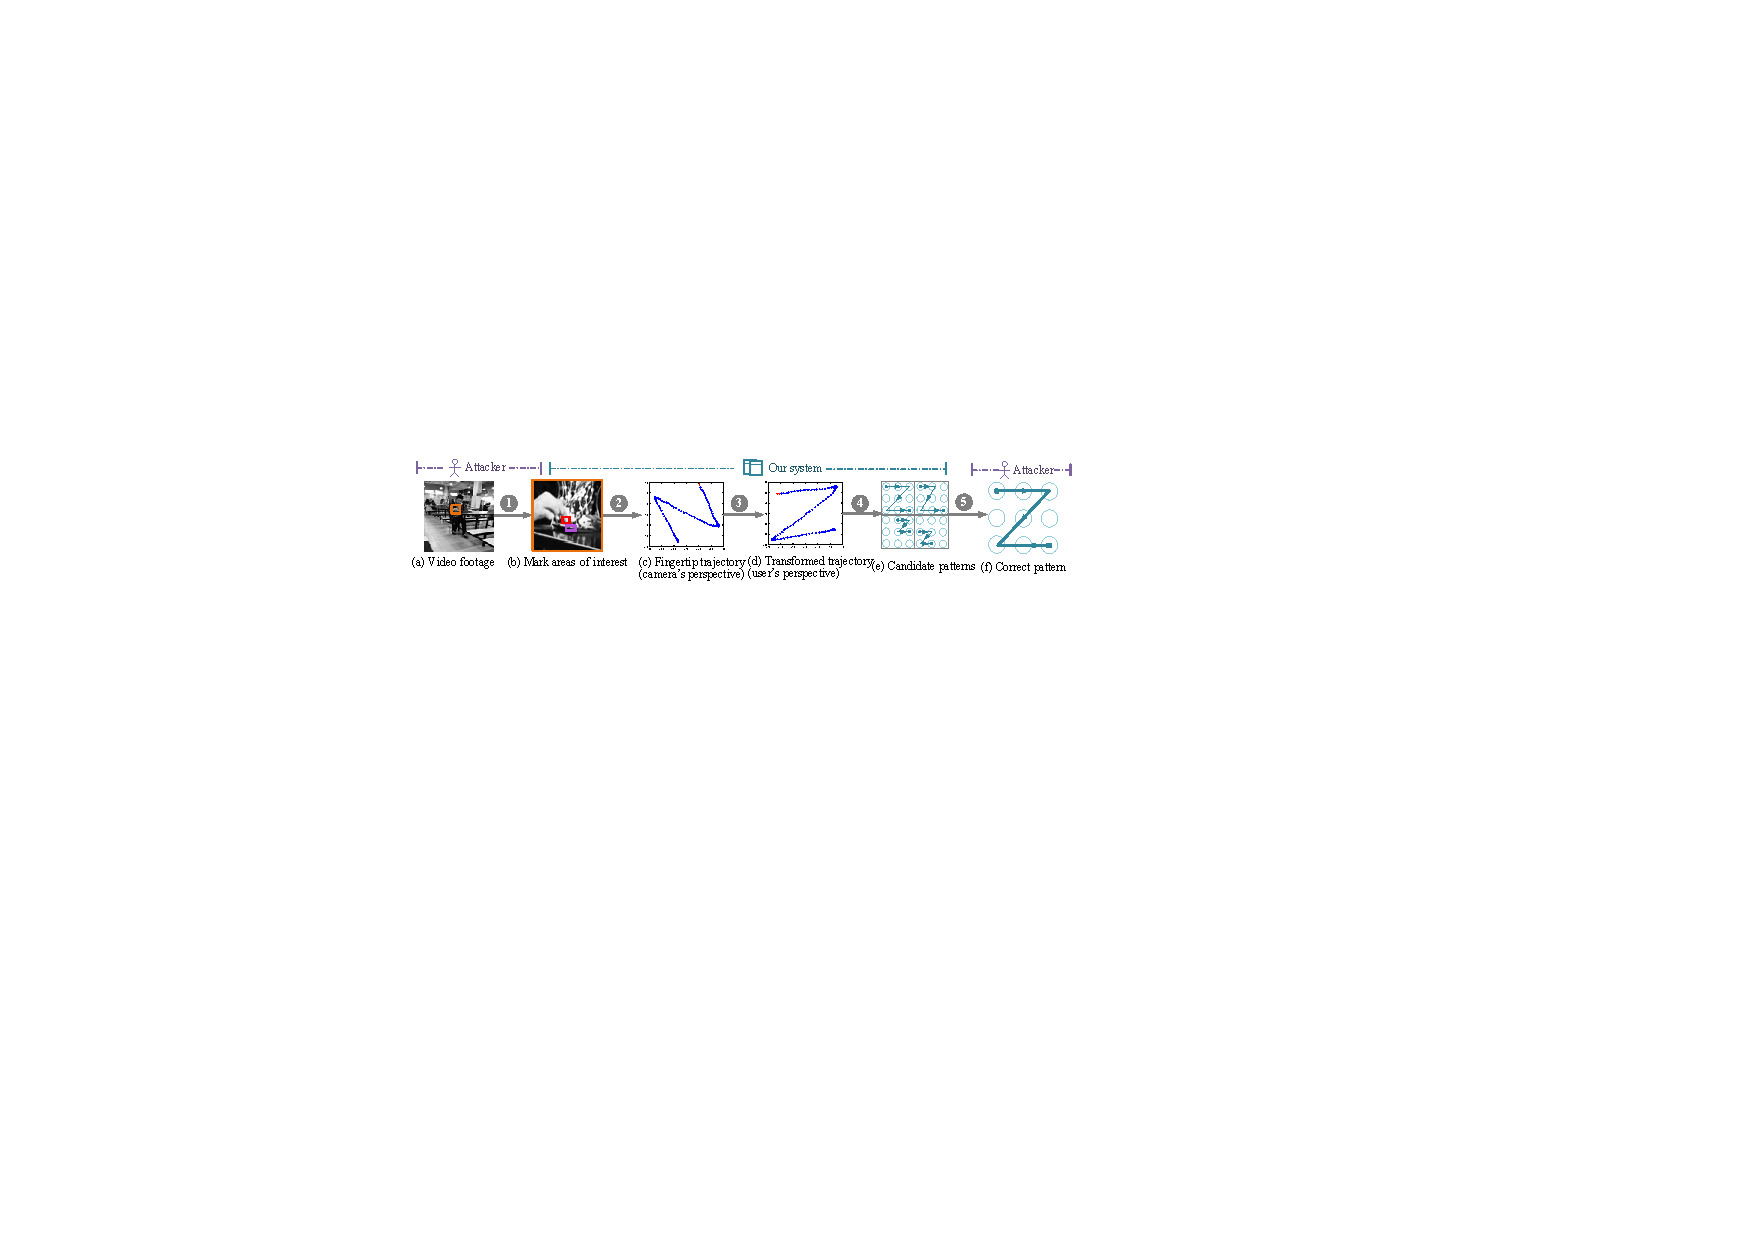
\includegraphics[width=\textwidth]{fig/overview.pdf}
    \vspace{-8mm}
    \caption{Overview of the attack.
     Our system takes in a video segment that records the unlocking process (a). The adversary first marks two areas of interest on the first video frame (b): one contains the fingertip involved in pattern drawing, and the other contains part of the device. Our system then tries to track the fingertip's location w.r.t. to the device.
     The tracking algorithm produces a fingertip movement trajectory from the camera's perspective (c) which is then transformed to the user's perspective (d). Finally, the resulted trajectory in (d) is mapped to several candidate patterns (e) to be tested on the target device (f). }
    \label{fig:fig2}
    \vspace{-5mm}
\end{figure*}

\vspace{-3mm}
\section{Background}
    \subsection{Android Pattern Lock}
    \label{section: android_pattern_lock}
        Pattern lock is widely used to protect sensitive information and perform authentication on
        Android touch-screen devices. Many users prefer to use pattern lock because they
        are easily to be recalled over alphanumeric characters~\cite{standing1970perception,Weiss2008PassShapes}.
        To unlock a device protected with pattern lock, the user is asked to draw a predefined sequence of connected dots on a pattern grid\footnote{In this paper we use the Android default pattern grid with $3 \times 3$ dots, unless otherwise stated.}.
        Figure~\ref{fig:fig2} (e) shows a pattern which consists of seven dots on a $3 \times 3$ grid.
        To form a
        pattern, the user starts by selecting one dot as the
        starting point and then swiping over multiple dots of the grid until the fingertip is lifted from the screen.
        %Essentially, pattern lock is a simplified variant of
%        the Pass-Go graphical based password scheme
%        \cite{biddle2012graphical}.
        There are several rules for creating an Android pattern: (1) a pattern must consist
        of at least four dots; (2) each dot can only be visited once; and (3) a previously unvisited dot will
        become visited if it is part of a horizontal, vertical or diagonal
        line segment of the pattern. Taking into account these constraints, the total number of possible patterns
        on a $3\times3$ grid is 389,112~\cite{uellenbeck2013quantifying}.
        Given the large number of possible patterns, performing brute-force attacks on
        Android pattern lock is ineffective, because the device will be
        automatically locked after five failed tries.
        Previous works also show that a brute-force attack is likely to fail on  patterns with complex
        structures~\cite{Kelley2012Guess,Mazurek2013Measuring}.

    %\vspace{-2mm}
    \subsection{Threat Model}
    \label{sec:scenarios}
        In our threat model, we assume an adversary wants to access some sensitive information from or to install malware on a
target device that is protected by pattern lock. This type of attacks is mostly likely to be performed by an attacker
who can physically access to the target device for a short period of time (e.g. via  attending a meeting or a party where
the user presents). To quickly gain access to the device, the attacker would like to obtain
the user's locking pattern in advance.

The attack starts from filming how the user unlocks the device. Video recording
can be done on-site or ahead of time. The video will then be processed to identify a small number of patterns to be
tested on the target device. Because filming can be carried out from a distance of as far as 2 meters using a
mobile phone camera and the camera does not need to directly face the target device (or about 9 meters using a digital single reflex camera), this activity often will not be
noticed by the user. Moreover, given that many users use the same pattern across devices and applications, the pattern
obtained from one device could also be used to break the user's other devices.  We want to stress that the goal of this paper is to
demonstrate the feasibility of a new attack and the countermeasure is left to our future work.

%\vspace{2mm}
\noindent \textbf{Examples of Filming Scenarios} 
Figure~\ref{fig:fig1} illustrates two day-to-day scenarios where filming can be
performed without raising suspicion to many users. For the two examples presented in Figure~\ref{fig:fig1}, the
filming camera had a left- or right-front view angle from the target device indoor or outdoor and did not directly face the screen of the target device. Due to the filming distance (2-3 meters), the recoded video typically does not have a clear vision of
the content displayed on the screen.  This observation can be confirmed by the video snapshot placing
alongside each scenario, where it is impossible to identify the content shown on the screen.


%Figure~\ref{fig:fig1} illustrates three scenarios where filming can be
%performed without raising suspicion to many users. For all the examples presented in Figure~\ref{fig:fig1}, the
%filming camera had a left- or right-front view angle from the target device and did not directly face the screen of the target device. Due to the filming distance (2-3 meters), the recoded video typically does not have a clear vision of
%the content displayed on the screen.  This observation can be confirmed by the video snapshot placing
%alongside each scenario, where it is impossible to identify the content shown on the screen.
%The examples given in Figure~\ref{fig:fig1} are some of the day-to-day
%scenarios where security of the user's device can be compromised under
%our attack.

%\vspace{2mm}
\noindent \textbf{Assumptions}
Our attack requires the video footage to have a vision of the user's
fingertip that was involved in pattern drawing as well as part of the device (e.g. an edge of a phone).
We believe this is a reasonable assumption because in practice many users often do not fully cover their fingers and the entire device when drawing a pattern.
This is particularly true when holding a large-screen device by hands.
To launch the
attack, the attacker needs to know the layout of the grid, e.g. whether it is
a $3 \times 3$ or a $6 \times 6$ grid. This can be simply decided by seeing target device.

%Our attack requires the video footage to have a vision of the user's
%fingertip that was involved in pattern drawing as well as part of the device (e.g. an edge of a phone).
%We believe this is a reasonable assumption because in practice many users often do not fully cover their fingers and the entire device when drawing a pattern.
%This is particularly true when holding a large-screen device by hands.
%To launch the
%attack, the attacker needs to know the layout of the grid, e.g. whether it is
%a $3 \times 3$ or a $6 \times 6$ grid. Our approach is to generate a set of
%candidate patterns for each of the Android pattern grids and the attacker can simply decide
%which set of candidate patterns to use after seeing the target device (at the time the
%layout of the grid will be available). However, unlike prior work on
%video-based attacks on keystroke based authentication~\cite{shukla2014beware}, our approach does not
%require having knowledge of the console's geometry. In other words, the size
%of the screen or the position of the pattern grid  on the screen does not
%affect the accuracy of our attack. We also assume the video does not need to
%capture any content displayed on the screen. This assumption makes previous
%video-based attacks on pattern lock~\cite{aviv2010smudge} inapplicable.
